% Panel captions --- included by medium-vertex-direction.tex
% Every value plotted is computed by validation/kernel/medium.py at draw
% time; nothing is transcribed.

\begin{figure}[!htbp]
\centering
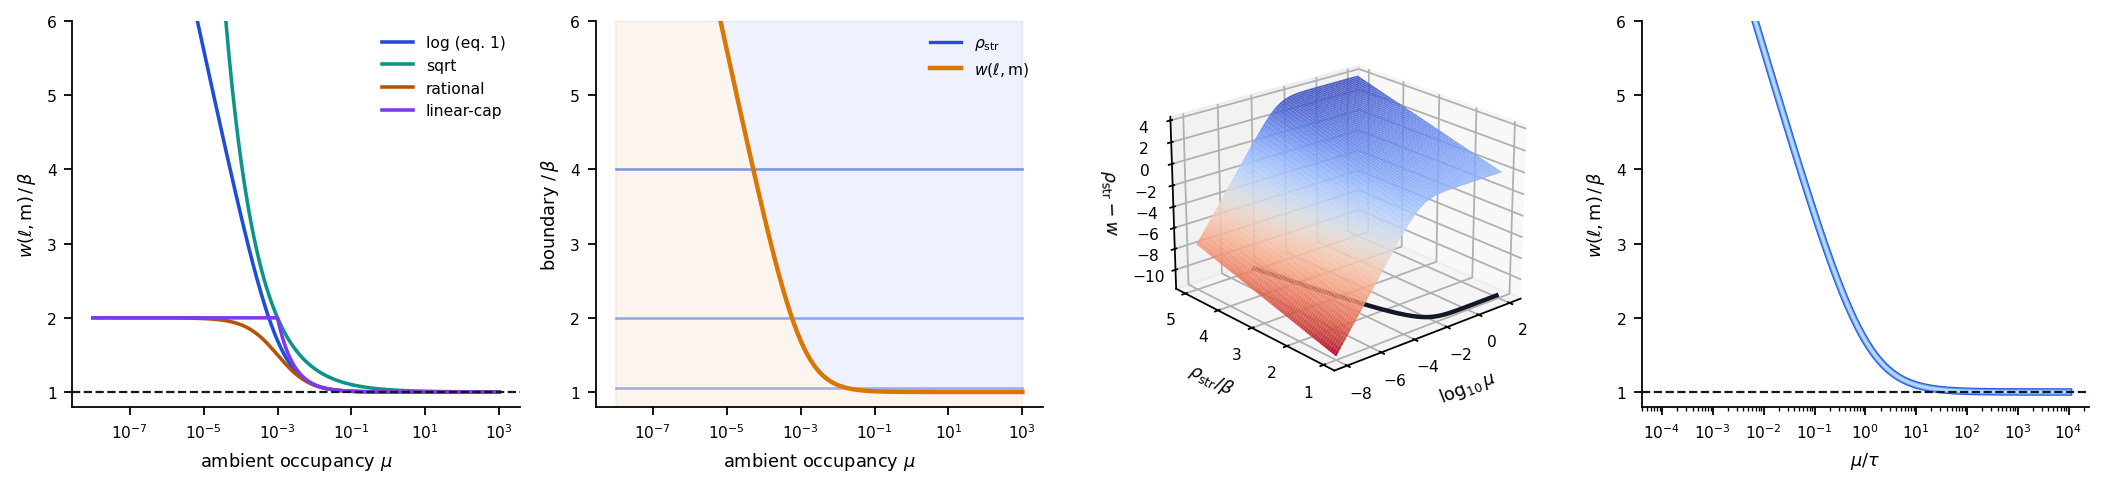
\includegraphics[width=\textwidth]{figures/panel_01_medium_weight.png}
\caption[The medium weight]{\textbf{The medium weight and its two
required properties.}
\textbf{(a)}~$w(\ell,\med)/\flo$ against ambient occupancy for the four
weight families of \Cref{rem:log}. All four are bounded below by $\flo$
(dashed) and strictly decreasing: abundance is cheap to individuate
against, scarcity expensive.
\textbf{(b)}~The two competing boundaries. Horizontal lines are
structural residues (independent of $\mu$); the falling curve is the
medium weight. Their crossing is the role boundary of
\Cref{def:solvent-role}.
\textbf{(c)}~The role margin $\res_{\mathrm{str}}-w(\ell,\med)$ over
occupancy and contact strength; the black contour is the zero level, the
role boundary itself.
\textbf{(d)}~Scale invariance. Three values of $\tau$ spanning four
decades collapse onto one curve when plotted against $\mu/\tau$,
confirming that $\tau$ and $\mu$ are not separately observable
(\Cref{def:reservoir}).}
\label{fig:panel1}
\end{figure}

\begin{figure}[p]
\centering
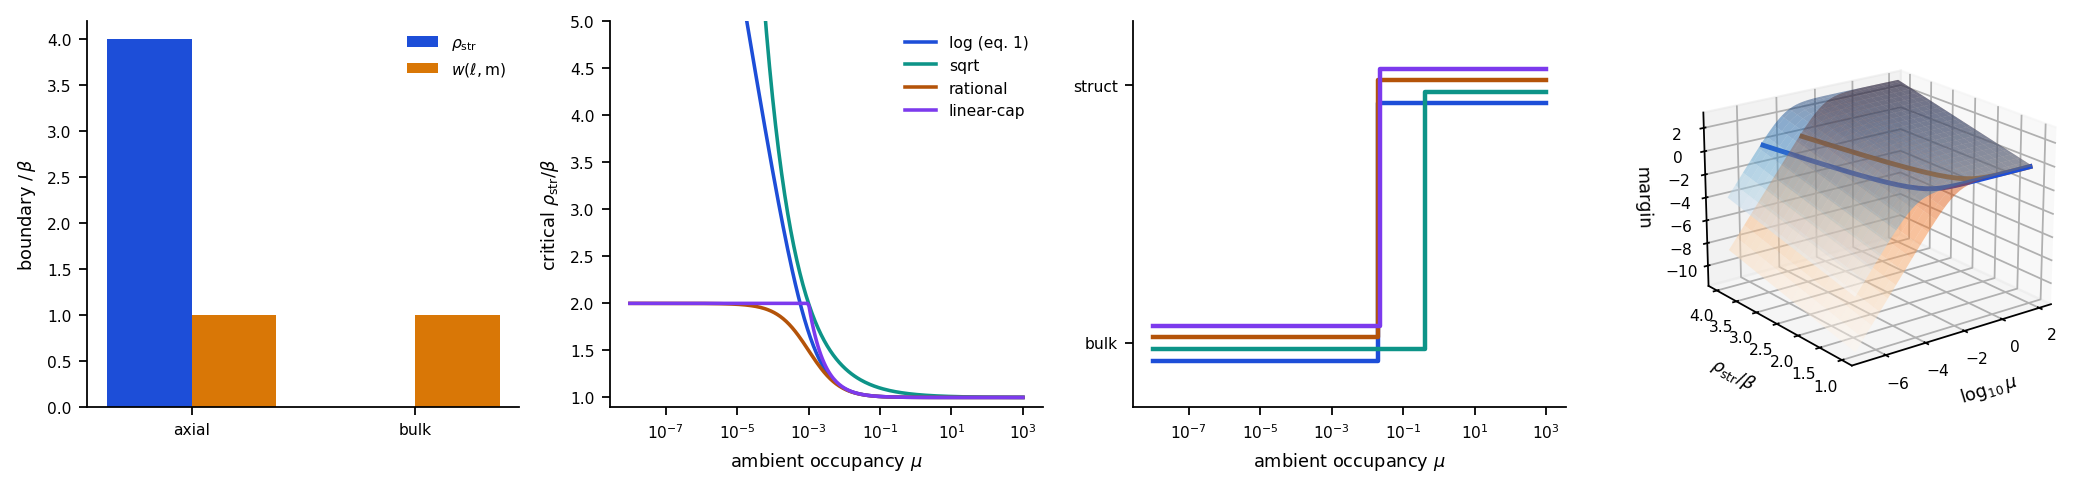
\includegraphics[width=\textwidth]{figures/panel_02_solvent_role.png}
\caption[Solvent role]{\textbf{Solvent role is derived, not annotated}
(\Cref{thm:solvent-role}).
\textbf{(a)}~The two boundaries for the CYP3A4 axial water and for a bulk
water of the same chemical identity. The axial water holds
$\res_{\mathrm{str}}=4\flo$ against the system; the bulk water holds
none. Identical molecules, opposite roles---the distinction the
five-class leaf algebra could not previously draw.
\textbf{(b)}~The critical structural residue at which a leaf becomes
structural, for each weight family.
\textbf{(c)}~Role against ambient occupancy at fixed weak contact
($1.05\flo$), traces offset for visibility. Every family flips
bulk~$\to$~structural exactly once and never back, which is
\Cref{thm:solvent-role}(iii); the flip is what makes the negative control
of \Cref{sec:refusal} non-vacuous.
\textbf{(d)}~The role margin for two exchange scales; the two zero
contours are the role boundaries, showing that $\tau$ moves the boundary
without changing its shape.}
\label{fig:panel2}
\end{figure}

\begin{figure}[p]
\centering
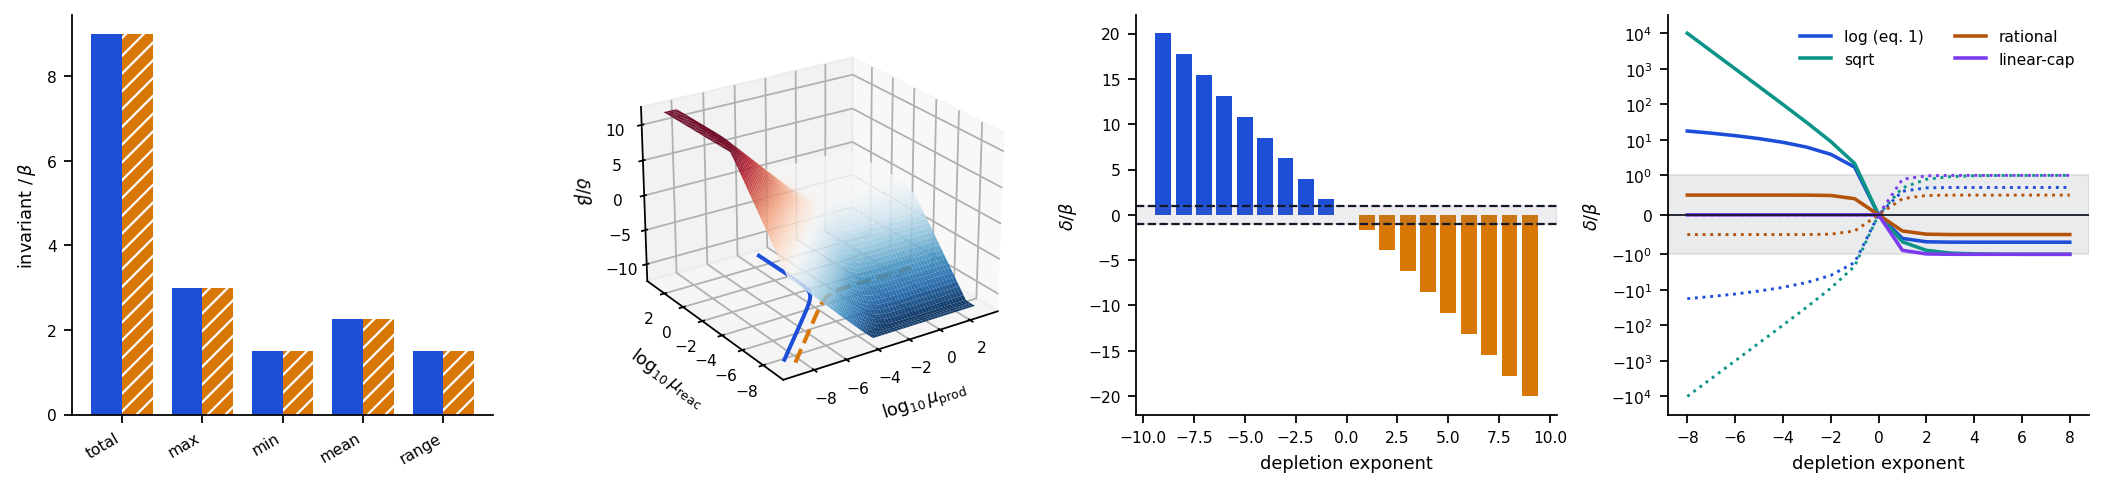
\includegraphics[width=\textwidth]{figures/panel_03_direction.png}
\caption[Reversal invariance and medium bias]{\textbf{The chain cannot
orient; the medium can.}
\textbf{(a)}~Five accumulated invariants of a residue chain and of its
reversal: total, maximum, minimum, mean and range. All five coincide
exactly, which is \Cref{lem:reversal}, and by \Cref{cor:no-orientation}
no statistic of the residues can therefore supply a direction.
\textbf{(b)}~The medium bias $\delta/\flo$ over independent depletion of
the product and reactant ends. The surface is antisymmetric about the
diagonal; the two contours at $\delta=\pm\flo$ bound the refusal region.
\textbf{(c)}~The two-sided sweep. Depleting a product drives the chain
forward (blue), depleting a reactant drives it in reverse (orange), and
the shaded band $\abs{\delta}\le\flo$ is undirected---all three cases of
\Cref{thm:direction} reached.
\textbf{(d)}~Antisymmetry across all four weight families (solid: $C$;
dotted: $C^{R}$), on a symmetric log axis. Every pair crosses at zero,
confirming $\Delta_{\med}(C^{R})=-\Delta_{\med}(C)$ independently of the
functional form.}
\label{fig:panel3}
\end{figure}

\begin{figure}[p]
\centering
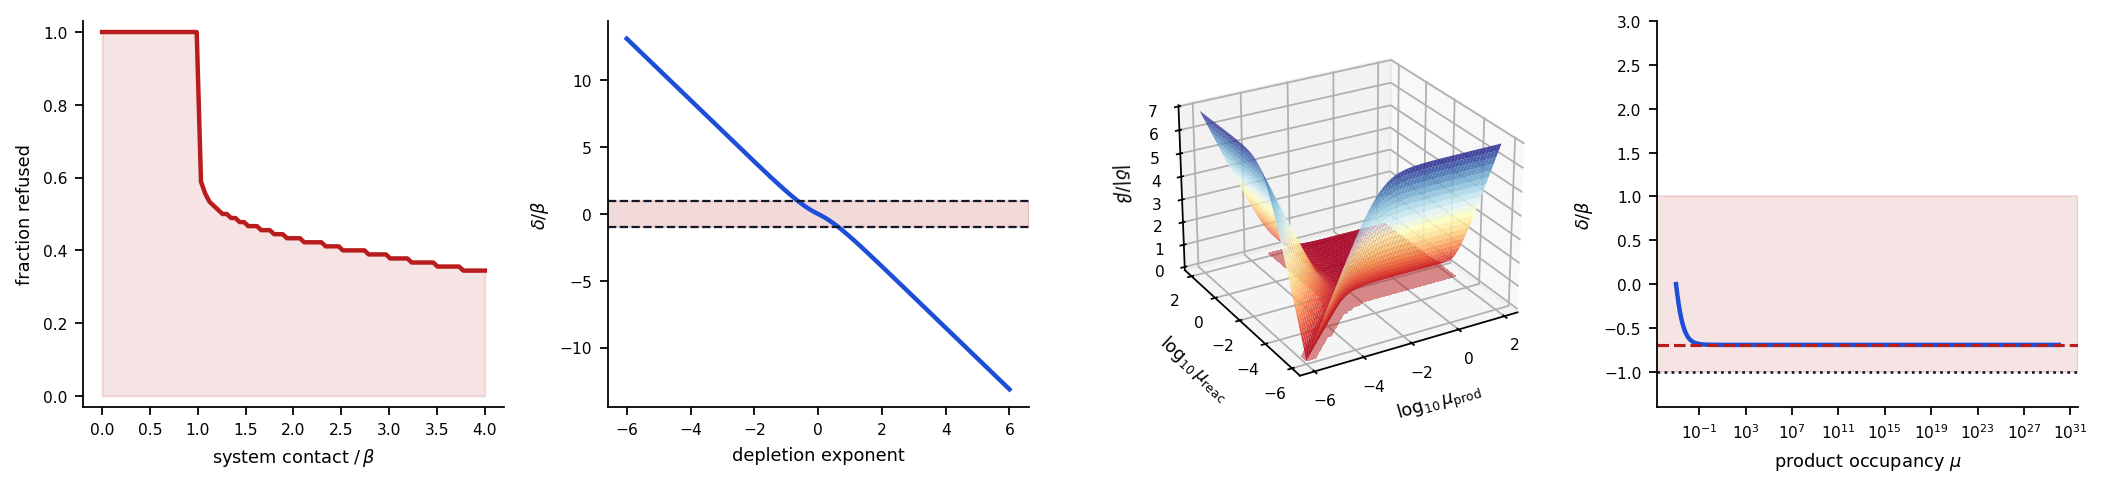
\includegraphics[width=\textwidth]{figures/panel_04_refusal.png}
\caption[The refusals]{\textbf{The framework's first refusals}
(\Cref{sec:refusal}).
\textbf{(a)}~Fraction of solvent leaves refused individuation against
contact strength. At zero system contact every leaf is refused, for every
occupancy---the negative control of \Cref{thm:refusal-nonvacuous}(i).
\textbf{(b)}~The orientation refusal band. Where
$\abs{\delta}\le\flo$ (shaded) the medium does not favour a direction by
an amount the receiver can resolve, and \shk{track} declines to orient.
\textbf{(c)}~$\abs{\delta}/\flo$ over both depletion axes. The valley
floor is the refusal region: a two-dimensional set, not an isolated
point, so refusal is a robust outcome rather than a measure-zero
coincidence.
\textbf{(d)}~The $\log 2$ ceiling. Flooding a single product with
occupancy spanning thirty orders of magnitude drives $\delta/\flo$ to
exactly $-\log 2 \approx -0.693$ (dashed) and never to the refusal
threshold $-1$ (dotted). Reversing a chain requires depleting a
\emph{reactant}, not flooding a product---an asymmetry of
\Cref{eq:medium-weight} found by a failing test rather than by
derivation.}
\label{fig:panel4}
\end{figure}

\begin{figure}[p]
\centering
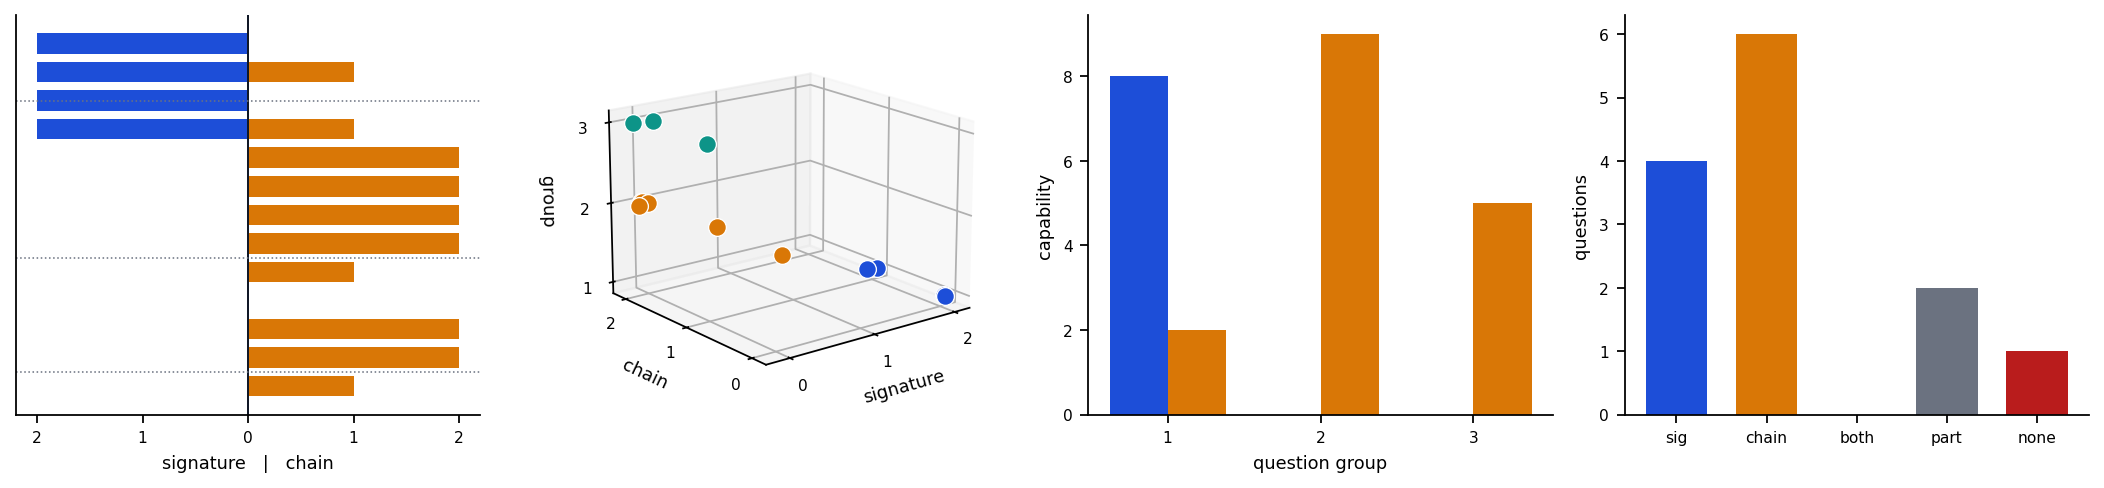
\includegraphics[width=\textwidth]{figures/panel_05_partition.png}
\caption[The representational partition]{\textbf{The competency questions
partition} (\Cref{sec:two-views}).
\textbf{(a)}~Per-question capability, signature view left, cut-chain view
right, grouped by the three question groups of
\citet{doerr2025limits}. Bars extend on one side or the other and almost
never on both.
\textbf{(b)}~The capability cube. Questions occupy the signature axis
(group~1) or the chain axis (group~2) but not the diagonal: no question
is answered fully by both views.
\textbf{(c)}~Group totals. Dominance reverses between group~1
(classification) and group~2 (mechanism), which is the block structure of
\Cref{tab:questions}.
\textbf{(d)}~The overlap statistic. Four questions are answered by the
signature alone, six by the chain alone, \emph{none} by both, two
partially and one by neither. The empty ``both'' column is the partition,
measured rather than asserted.}
\label{fig:panel5}
\end{figure}
